\documentclass[a4paper]{report}

\usepackage[T1]{fontenc}

\usepackage[margin=3.5cm, includeheadfoot]{geometry}
\usepackage{adjustbox}

\usepackage[scale=0.85]{sourcecodepro}

\usepackage{tikz}
\usetikzlibrary{positioning,fit}

\usepackage{booktabs}
\usepackage{listings}

\usepackage[backend=biber]{biblatex}

\addbibresource{resources.bib}

\lstset{%
	language=Eiffel,
	basicstyle=\ttfamily,
	keywordstyle=\color{blue},
	showstringspaces=false, tabsize=4,
	deletekeywords={},
	morekeywords={%
		True, False, Precursor,
		MANAGED_POINTER, FILE, RAW_FILE, NATURAL_64, READABLE_STRING_GENERAL,
		TAR_HEADER, TAR_CONST, ARCHIVE,
		FILE_STORAGE_BACKEND, STORAGE_BACKEND,
		ARCHIVABLE, FILE_ARCHIVABLE, DIRECTORY_ARCHIVABLE,
		UNARCHIVER, FILE_UNARCHIVER, DIRECTORY_UNARCHIVER,
		HEADER_SAVE_UNARCHIVER, HEADER_PRINT_UNARCHIVER
	},
}

\begin{document}

\chapter{Overview}
The etar library provides support for archiving data using the pax/tar format.

\section{Concepts}
\subsection{Archive}
An archive is a series of blocks of size 512 bytes. An entry consists of exactly
one header block, followed by zero or more payload blocks. At the end of the
archive there are two consecutive blocks with all zero bytes.

\begin{figure}[h]
	\begin{center}
		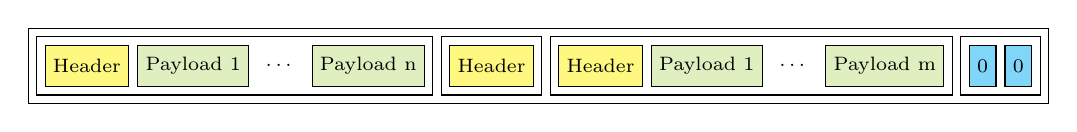
\begin{tikzpicture} [
		every node/.style={inner sep=1mm, node distance=1mm, minimum height=1.5em,
			font=\scriptsize, anchor=west, rectangle},
		entry/.style={draw=black},
		header/.style={draw=black, fill=yellow!50},
		payload/.style={draw=black, fill=green!50!orange!25},
		null/.style={draw=black, fill=cyan!50}
	]
	\node (hdr1) [header] {Header};
	\node (pl11) [payload, right=of hdr1.east] {Payload 1};
	\node (d1) [right=of pl11.east] {\dots};
	\node (pl1n) [payload, right=of d1.east] {Payload n};
	\node (e1) [entry, fit={(hdr1) (pl11) (d1) (pl1n)}] {};

	\node (hdr2) [header, right=of e1.east, xshift=1mm] {Header};
	\node (e2) [entry, fit={(hdr2)}] {};

	\node (hdr3) [header, right=of e2.east, xshift=1mm] {Header};
	\node (pl31) [payload, right=of hdr3.east] {Payload 1};
	\node (d3) [right=of pl31.east] {\dots};
	\node (pl3n) [payload, right=of d3.east] {Payload m};
	\node (e3) [entry, fit={(hdr3) (pl31) (d3) (pl3n)}] {};

	\node (n1) [null, right=of e3.east, xshift=1mm] {0};
	\node (n2) [null, right=of n1.east] {0};

	\node (n) [entry, fit={(n1) (n2)}] {};

	\node (archive) [entry, fit={(e1) (e2) (e3) (n)}] {};

\end{tikzpicture}

	\end{center}
	\caption{Structure of an archive}
\end{figure}

\section{Error Handling}
API still unstable

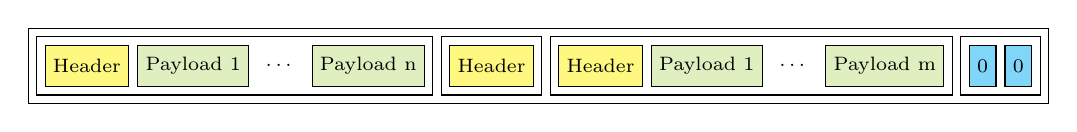
\begin{tikzpicture} [
		every node/.style={inner sep=1mm, node distance=1mm, minimum height=1.5em,
			font=\scriptsize, anchor=west, rectangle},
		entry/.style={draw=black},
		header/.style={draw=black, fill=yellow!50},
		payload/.style={draw=black, fill=green!50!orange!25},
		null/.style={draw=black, fill=cyan!50}
	]
	\node (hdr1) [header] {Header};
	\node (pl11) [payload, right=of hdr1.east] {Payload 1};
	\node (d1) [right=of pl11.east] {\dots};
	\node (pl1n) [payload, right=of d1.east] {Payload n};
	\node (e1) [entry, fit={(hdr1) (pl11) (d1) (pl1n)}] {};

	\node (hdr2) [header, right=of e1.east, xshift=1mm] {Header};
	\node (e2) [entry, fit={(hdr2)}] {};

	\node (hdr3) [header, right=of e2.east, xshift=1mm] {Header};
	\node (pl31) [payload, right=of hdr3.east] {Payload 1};
	\node (d3) [right=of pl31.east] {\dots};
	\node (pl3n) [payload, right=of d3.east] {Payload m};
	\node (e3) [entry, fit={(hdr3) (pl31) (d3) (pl3n)}] {};

	\node (n1) [null, right=of e3.east, xshift=1mm] {0};
	\node (n2) [null, right=of n1.east] {0};

	\node (n) [entry, fit={(n1) (n2)}] {};

	\node (archive) [entry, fit={(e1) (e2) (e3) (n)}] {};

\end{tikzpicture}

\chapter{TAR\_HEADER}
A \lstinline|TAR_HEADER| instance contains all metadata, tarfiles store. The
parts about size, mtime and typeflag are based on \cite[Shell \& Utilities - pax]{POSIX:2008}.

\section{Metadata}
\subsection{filename}
path to the file

\subsection{mode}
Traditional UNIX style mode (0777, 0644, \dots).

\subsection{user\_id}
User ID of the file owner.

\subsection{group\_id}
Group ID of the file group.

\subsection{size}
For files this contains the size in bytes. In case the header does not belong
to a file, this is either zero or unspecified by the posix standard, so leaving
it at its default value (0) is a good choice.

The only exception are directories, for which a non-zero size indicates the
maximal number of bytes that this directory is able to hold (if supported by
the OS). If the size is zero there is no such limit (or no OS support).

\subsection{mtime}
Modification time of the file at archiving time, measured in unix time (seconds
since 00:00:00 UTC on 1 January 1970).

\subsection{typeflag}
Indicates what payload type this header follows. The following values are
standardized:
\begin{itemize}
	\item['0'] Regular files ('\%U' is allowed for backward compatibilty but
		should not be used)
	\item['1'] Hardlink (only allowed if the content was archived in an earlier
		entry)
	\item['2'] Symlink
	\item['3'] Character special device
	\item['4'] Block special device
	\item['5'] Directory
	\item['6'] FIFO
	\item['7'] Reserved for files to which an implementation has associated some
		high-performance attribute. May treat it as regular file.
	\item['A'-'Z'] Reserved for custom implementations
	\item Everything else is reserved for future standardization.
\end{itemize}

\subsection{linkname}
Target (pointee) of a link-type entry.

\subsection{user\_name}
Username of the file owner.

\subsection{group\_name}
Groupname of the file group.

\subsection{device\_major}
Device major number of a character or block device.

\subsection{device\_minor}
Device minor number of a character or block device.

\chapter{STORAGE\_BACKEND}
\lstinline;STORAGE_BACKEND; provides a unified interface for different storage
methods an archive could use. Currently the only implementation is
\lstinline;FILE_STORAGE_BACKEND;, providing support for archives that are stored
in a file.

\section{FILE\_STORAGE\_BACKEND}
A \lstinline;FILE_STORAGE_BACKEND; is either created from a file with
\lstinline;make_from_file; or from a filename with
\lstinline;make_from_filename;.

\section{Implementing a Custom STORAGE\_BACKEND}
To implement a custom \lstinline;STORAGE_BACKEND;, one has to implement the
following features:

\subsection{Creation Procedures}
If \lstinline;default_create; is redefined, \lstinline;Precursor; must be
called. Every other creation procedure should call \lstinline;default_create;.

\subsection{open\_read}
\lstinline;open_read;\\
Open backend for read access. Reading should start from the beginning.

\subsection{open\_write}
\lstinline;open_write;\\
Open backend for write access. Writing should start from the beginning.

\subsection{close}
\lstinline;close;\\
Close backend.

\subsection{archive\_finished}
\lstinline;archive_finished: BOOLEAN;\\
Indicate whether the next two blocks contain the end-of-archive indicator
(only zero bytes). The next \lstinline;read_block; calls should not skip these
two blocks but read them again (not necessarily from the backend again, the
implementation is free to chache these blocks).
\lstinline;archive_finished; should return \lstinline;True; too, if an error
occured (or occurs while checking for the end-of-archive indicator), does not
have enough blocks available or if the backend is closed.

\subsection{block\_ready}
\lstinline;block_ready: BOOLEAN;\\
Indicate whether there is a block that can be read with \lstinline;last_block;
\lstinline;False; if an error occured.


\subsection{is\_readable}
\lstinline;is_readable: BOOLEAN;\\
Indicates whether this backend can be read from. If an error occured, this has
to return \lstinline;False;

\subsection{is\_writable}
\lstinline;is_writable: BOOLEAN;\\
Indicates whether this backend can be written to. If an error occured, this has
to return \lstinline;False;

\subsection{is\_closed}
\lstinline;is_closed: BOOLEAN;\\
Indicates whether this backend is closed.

\subsection{read\_block}
\lstinline;read_block;\\
Read next block from backend. If there are not enough bytes for a full block, an
error should be reported.

\subsection{last\_block}
\lstinline;last_block: MANAGED_POINTER;\\
Last block that was read.

\subsection{write\_block}
\lstinline;write_block (block: MANAGED_POINTER);\\
Write \lstinline;block; to the backend (starting from the beginning).

\subsection{finalize}
\lstinline;finalize;\\
Write the end-of-archive indicator and close backend.

\chapter{ARCHIVABLE}
Everything that one wants to add to an archive has to inherit from
\lstinline;ARCHIVABLE;, which provides an interface that \lstinline;ARCHIVE;
uses to write it. The etar library provides two implementations.

\section{FILE\_ARCHIVABLE}
\lstinline;FILE_ARCHIVABLE; allows to archive plain files. A client has to
provide a \lstinline;FILE; for which the \lstinline;FILE_ARCHIVABLE; will be
created.

\section{DIRECTORY\_ARCHIVABLE}
\lstinline;DIRECTORY_ARCHIVABLE; allows to archive a directory (without its
contents!). On creation the client has to provide a \lstinline;FILE; (!) (for
which \lstinline;is_directory; holds).

\section{Implementing a custom ARCHIVABLE}
To implement a custom \lstinline;ARCHIVABLE;, one has to implement the following
features:

\subsection{Creation Procedures}
There is nothing to consider for creation procedures.

\subsection{required\_blocks}
\lstinline;required_blocks: INTEGER; \\
Has to return how many blocks are needed to archive the payload.

\subsection{header}
\lstinline;header: TAR_HEADER; \\
Has to return a \lstinline;TAR_HEADER; object suitable for the archivable type
and the payload.

\subsection{write\_block\_to\_managed\_pointer}
\lstinline|write_block_to_managed_pointer (p: MANAGED_POINTER; a_pos: INTEGER)| \\
Has to write the next block to \lstinline;p; (writing should start at position
\lstinline;a_pos;). This feature has to increase \lstinline;written_blocks; by
one.
In case the payload does not fill a whole block, it has to be padded to full
block size (\lstinline|{TAR_CONST}.tar_block_size|).

\subsection{write\_to\_managed\_pointer}
\lstinline|write_to_managed_pointer (p: MANAGED_POINTER; a_pos: INTEGER)| \\
Has to write the whole payload (padded to
\lstinline|{TAR_CONST}.tar_block_size|) bytes. Calling this feature must not
change the state of blockwise writing.

\subsection{Utility Features}
To implement the features listed above, the following utility features are
provided:

\subsubsection{Padding}
To pad a block to some size, one can use
\lstinline|pad (p: MANAGED_POINTER; a_pos, n: INTEGER)|\\
It pads a given block \lstinline;p; with \lstinline;n; zero-bytes, starting
from position \lstinline;a_pos;. If \lstinline|n| is zero, nothing will be
padded (but it's legal to call it with \lstinline|n = 0|).

\subsection{End of Payload}
To determine whether the last payload block was written, one can compare
\lstinline;required_blocks; with \lstinline;written_blocks;

\subsection{Bytes to Blocks}
The feature \lstinline|needed_blocks (n: INTEGER): INTEGER)| can be used to
determine how many blocks are required to store \lstinline;n; bytes.

\chapter{UNARCHIVER}
\lstinline;UNARCHIVER; is the central piece for unarchiving. \lstinline;ARCHIVE;
will parse the header and search for the last registered (!)
\lstinline;UNARCHIVER; that can unarchive the payload that belongs to the
header. This \lstinline;UNARCHIVER; will then be initialized with the header
and be passed blocks until it indicates that unarchiving finished.

etar provides two predefined \lstinline;UNARCHIVER;s

\section{FILE\_UNARCHIVER}
\lstinline;FILE_UNARCHIVER; accepts all headers that have a typeflag for a
regular file ('0' and '\%U'). It will create a \lstinline;RAW_FILE; and copy all
payload blocks to it until \lstinline;size; bytes are written (indicated by the
header). Additionally it will try to set the metadata according to the header.

\section{DIRECTORY\_UNARCHIVER}
\lstinline;DIRECTORY_UNARCHIVER; accepts all headers that have the directory
typeflag ('5'). It will create a new directory and try to set the metadata
according to the header.

\section{Implementing a Custom UNARCHIVER}
To implement a custom \lstinline;UNARCHIVER;, one has to implement the following
features. Additional examples of custom \lstinline;UNARCHIVER;s can be found in
the examples directory (minipax's \lstinline;HEADER_SAVE_UNARCHIVER; and
tar\_ls' \lstinline;HEADER_PRINT_UNARCHIVER;).

\subsection{Creation Procedures}
All creation procedures have to call \lstinline;default_create; either using
\lstinline;Precursor; or by calling it directly.

\subsection{required\_blocks}
\lstinline;required_blocks: INTEGER;\\
Has to return the number of blocks that are required to unarchive the payload
that belongs to this header.

\subsection{can\_unarchive}
\lstinline;can_unarchive (a_header: TAR_HEADER): BOOLEAN;\\
Indicates whether \lstinline;a_header; can be unarchived by this
\lstinline;UNARCHIVER; type. This is the function, \lstinline;ARCHIVABLE; uses
to determine which \lstinline;UNARCHIVER; it should chose.

\subsection{unarchive\_block}
\lstinline|unarchive_block (a_block: MANAGED_POINTER; a_pos: INTEGER)| \\
Takes a block and unarchives its contents. The block starts at
\lstinline;a_pos;. This feature unarchives at most
\lstinline;{TAR_CONST}.tar_block_size; blocks. It has to increase
\lstinline;unarchived_blocks; by one.

\subsection{do\_internal\_initialization}
Initialize internal structures (only the ones this \lstinline;UNARCHIVER;
introduces). It is called automatically by \lstinline;initialize;.

\subsection{Utility Features}
To implement the features listed above, the following utility features are
provided.

\subsubsection{Bytes to Blocks}
The feature \lstinline|needed_blocks (n: NATURAL_64): NATURAL_64)| can be used
to determine how many blocks are required to store \lstinline;n; bytes.

\subsection{UID to Username}
To convert a uid to a username, \lstinline|file_owner (uid: INTEGER): STRING|
can be used.

\subsection{GID to Groupname}
To convert a gid to a groupname, \lstinline|file_group (gid: INTEGER): STRING|
can be used.


\printbibliography[heading=bibintoc]

\end{document}
